\newpage
\section*{MÉTODOS}
\addcontentsline{toc}{section}{MÉTODOS}
\par\refstepcounter{section}
\subsection{Campos de fuerza basados en conocimiento}
\par
Los potenciales de fuerza media utilizados y derivados en este trabajo parte del supuesto de que las fuerzas encontradas en sistemas moleculares grandes son excesivamente complejas, por lo tanto la única fuente de información confiable son estructuras resueltas en su estado nativo y en equilibrio. 
Si la extracción de información es exitosa, el campo de fuerza será capaz de determinar correctamente si un motivo en una molécula es nativo o no. 
Esta es la llamada aproximación deductiva o \textit{knowledge-based} de un potencial de fuerza 
media. (\cite{Sippl1993})
\par
Un potencial de fuerza media parte de la ley inversa de Boltzmann:
\begin{equation}
E_{ijkl} = -kT\log(f_{ijkl}) + kT\log Z \label{ec:boltz1}
\end{equation}
La función de energía E\textsubscript{ijkl} es el llamado potencial de fuerza media. 
La variable \textit{f} es la frecuencia relativa de un cierto estado al fijar las variables i, j, k, l en 
los sistemas observados en nuestra base de datos. 
\textit{Z} representa la función de partición y no puede ser calculada experimentalmente, y se le da el 
valor de 1 (\cite{Sippl1993}). 
La ecuación~\eqref{ec:boltz1}  entonces toma la forma:
\begin{equation}
E_{ijkl} = -kT\log(f_{ijkl}) \label{ec:boltz2}
\end{equation}
\par
ero para utilizar exitosamente la ley inversa de Boltzmann es necesario también definir un sistema de referencia apropiado. 
Este se obtiene promediando un conjunto elegido de variables del sistema, como por ejemplo k y l.
Esto nos permite extraer una característica energética general de los sistemas, las cuáles también se definen como un potencial de energía:
\begin{equation}
E_{kl} = -kT\log(f_{kl}) \label{ec:boltzref}
\end{equation}
\par
Con esto, ahora podemos obtener el valor neto del potencial de fuerza media:
\begin{equation}
\Delta E^{ij}_{kl} = E^{ij}_{kl} - E_{kl} = -kT\log \left( \frac{f^{ij}_{kl}}{f_{kl}} \right) \label{ec:boltzref2}
\end{equation}
\par
En el contexto de este trabajo, nuestras variables \textit{i} y \textit{j} indican el tipo de interacción entre dos átomos (en el caso de los potenciales SASA, solo se usa la variable \textit{i}), mientras que \textit{k} y \textit{l} indican distancia en la secuencia de residuos y el \textit{bin} de la variable geométrica a analizar, que puede ser la distancia, BSASA o SASA.
Se aplica también un factor de corrección para números bajos de observaciones en la base de datos, sugerido en \cite{Sippl1990}. 
Así, cuando en función de \textit{l} la ecuación final toma la forma:
\begin{equation}
\Delta E^{ij}_{k}(l) = RT\log \left[1 + M_{ijk}\sigma\right] - RT\log \left[ 1 + M_{ijk}\sigma \frac{f^{ij}_{k}(l)}{f_{k}(l)} \right] \label{ec:finalboltz}
\end{equation}
Donde \textit{M\textsubscript{ijk}} corresponde al número de observaciones de interacciones del par al nivel de separación \textit{k}, y $\sigma$ al peso que se le da a cada observación. 
En este trabajo se utilizó $\sigma$ = 1/50. (\cite{Sippl1990,Melo1997})


\subsection{Determinación de tipos atómicos}
\par
Para los potenciales en proteínas, se utilizaron 40 tipos atómicos compartidos para los 20 aminoácidos.
Esto es debido a que existen 98 tipos atómicos no equivalentes en total, lo que resultaría en una base de datos con muy pocos datos para cada par de interacciones (\cite{Melo1997}).
Las definiciones se pueden ver en la tabla~\ref{table:atomprotdef}.
%tabla tipos
\newpage
\cleardoublepage
%\addcontentsline{lot}{table}{Definición de tipos atómicos para proteínas}
\begin{table}[!htp]
\begin{tabular}{ p{40pt} p{380pt} }
  \hline
  Tipo atómico & Lista de átomos \\
  \hline
  1 & \Ca\ para todos los aminoácidos excepto Glicina \\
  2 & \Ca\ Glicina \\
  3 & N para todos los aminoácidos excepto Prolina \\
  4 & C para todos los aminoácidos \\
  5 & O para todos los aminoácidos \\
  6 & Ala-\Cb, Ile-\Cgii, Ile-\Cd, Leu-\Cdi, Leu-\Cdii, Thr-\Cg, Val-\Cgi, Val-\Cgii \\
  7 & Ile-\Cb, Leu-\Cg, Val-\Cb \\
  8 & Arg-\Cb, Arg-\Cg, Asn-\Cb, Asp-\Cb, Gln-\Cb, Gln-\Cg, Glu-\Cb, Glu-\Cg, His-\Cb, Ile-\Cgi, Leu-\Cb, Lys-\Cb, Lys-\Cg, Lys-\Cd, Met-\Cb, Phe-\Cb, Pro-\Cb, Pro-\Cg, Trp-\Cb, Tyr-\Cb \\
  9 & Met-S\textsubscript{\text{\textdelta}} \\
 10 & Pro-N \\
 11 & Phe-\Cg, Trp-\Cdii, Tyr-\Cg \\
 12 & Phe-\Cdi, Phe-\Cdii, Phe-\Cei, Phe\Ceii, Phe-\Cz, Trp-\Ceiii, Trp-\Cz, Trp-\Cziii, Trp-\Cetaii, Tyr-\Cdi, Tyr-\Cdii, Tyr-\Cei, Tyr-\Ceii \\
 13 & Trp-\Cg \\
 14 & Trp-\Ceii \\
 15 & Ser-\Cb \\
 16 & Ser-O\textsubscript{\text{\textgamma}}, Thr-O\textsubscript{\text{\textgamma}} \\
 17 & Thr-\Cb \\
 18 & Asn-N\textsubscript{\text{\textdelta}2}, Gln-N\textsubscript{\text{\textepsilon}2} \\
 19 & Cys-S\textsubscript{\text{\textgamma}} \\
 20 & Lys-N\textsubscript{\text{\textzeta}} \\
 21 & Arg-\Cz \\
 22 & Arg-N\textsubscript{\text{\texteta}1}, Arg-N\textsubscript{\text{\texteta}2} \\
 23 & His-\Cg \\
 24 & His-\Cdii, Trp-\Cdi \\
 25 & His-N\textsubscript{\text{\textepsilon}2} \\
 26 & His-\Cei \\
 27 & Asp-\Cg, Glu-\Cd \\
 28 & Asp-O\textsubscript{\text{\textdelta}1}, Asp-O\textsubscript{\text{\textdelta}2}, Glu-O\textsubscript{\text{\textepsilon}1}, Glu-O\textsubscript{\text{\textepsilon}2} \\
 29 & Cys-\Cb, Met-\Cg \\
 30 & Met-\Ce \\
 31 & Tyr-\Cz \\
 32 & Pro-\Cd \\
 33 & Asn-\Cg, Gln-\Cd \\
 34 & Asn-O\textsubscript{\text{\textdelta}1}, Gln-O\textsubscript{\text{\textepsilon}1} \\
 35 & Lys-\Ce \\
 36 & Arg-N\textsubscript{\text{\textepsilon}} \\
 37 & Arg-\Cd \\
 38 & His-N\textsubscript{\text{\textdelta}1} \\
 39 & Trp-N\textsubscript{\text{\textepsilon}1} \\
 40 & Tyr-O\textsubscript{\text{\texteta}} \\
 \hline
\end{tabular}
\caption[Definiciones de átomos para proteínas]{Definiciones de átomos pesados utilizadas para potenciales en proteínas. Átomos del tipo 10 son convertidos al tipo 3 si son el primer residuo de una cadena proteíca.}
\label{table:atomprotdef}
\end{table}
%fin tabla tipos
\newpage
\clearpage
\par
En el caso de los potenciales para ADN y ARN, se utilizaron 23 tipos atómicos distintos descritos por \cite{Capriotti2011} para moléculas de ARN. A estos se agregaron dos tipos más, 24 y 25, correspondientes a los carbonos C5 y C7 (nombres IUPAC) del nucleótido timina.
Estas definiciones están en la tabla~\ref{table:atomnadef}.
%comienzo tabla nucleótidos
\newpage
\cleardoublepage
\begin{table}[!htp]
\begin{tabular}{p{40pt} p{380pt}}
  \hline \\
  Tipo atómico & Lista de átomos (nombres IUPAC) \\
  \hline \\
  1 & OP1, OP2, OP3 para todos los nucleótidos \\
  2 & P para todos los nucleótidos \\
  3 & O5' para todos los nucleótidos \\
  4 & C5' para todos los nucleótidos \\
  5 & C5', C3', C2' para todos los nucleótidos \\
  6 & O2', O3' terminales \\
  7 & C1' para todos los nucleótidos \\
  8 & O4' para todos los nucleótidos \\
  9 & N1 pirimidinas; N9 purinas \\
 10 & C8 purinas \\
 11 & N3, N7 en purinas; N1 en A; N3 en \\
 12 & C5 purinas \\
 13 & C4 purinas \\
 14 & C2 en A \\
 15 & C6 en A; C4 en C \\
 16 & N6 en A; N4 en C; N2 en G \\
 17 & C2 en G \\
 18 & C6 en G; C4 en U,T \\
 19 & O2 pirimidinas; O6 en G; O4 en U,T \\
 20 & C2 pirimidinas \\
 21 & C6 pirimidinas \\
 22 & C6 pirimidinas \\
 23 & N1 en G; N3 en U,T \\
 24 & C5 en T \\
 25 & C7 en T \\
 \hline
\end{tabular}
\caption[Definiciones de átomos para ADN y ARN]{Definiciones de átomos pesados utilizadas para potenciales en ARN y ADN. 
Se consideran tanto nucleótidos como deoxinucleótidos.}
\label{table:atomnadef}
\end{table}
%fin tabla nucleotidos
\newpage
\clearpage
\subsection{Derivación de potenciales basados en distancias y conteos de átomos}
\subsubsection{Derivación de potenciales basados en distancias}
\par
La derivación de los potenciales se hizo utilizando un programa escrito en C++, dada la gran cantidad de datos a procesar.
Se utilizaron los mismos parámetros de derivación utilizados en \cite{Melo1998} para los potenciales en proteínas, por lo que solo se consideran interacciones entre átomos a 7 \si{\angstrom} de distancia y separados por un mínimo de 13 residuos si los átomos pertenecen a una misma cadena.

\par
Para los potenciales en ARN y ADN, se utilizan los parámetros similares a los utilizados en \cite{Capriotti2011}, donde se usan 6 funciones distintas. Las funciones para ADN consideran interacciones a 7 \si{\angstrom} de distancia, mientras que las para ARN consideran interacciones hasta 20 \si{\angstrom}.
Esto último se debe a que el potencial de distancia RASP se usa como base para facilitar las comparaciones.
Las primeras 5 funciones solo consideran como interacciones átomos que están exactamente a 1, 2, 3, 4 y 5 residuos de distancia más cualquier interacción en otra cadena. 
La última función solo considera interacciones a 6 o más residuos de distancia.
Las distancias entre los átomos están discretizadas en 35 clases uniformes de 0.2 \si{\angstrom}, paso necesario para obtener datos de frecuencia.
Los pasos descritos en el algoritmo~\ref{alg:deralgo1} son los mínimos necesarios para la generación del potencial. 
Las variables \textit{Radius, Lmin, Lmax, Nclases y Sigma} corresponden respectivamente a la distancia máxima de interacción, la distancia mínima entre residuos de una misma cadena que se considera como interacción, la distancia máxima entre residuos de una misma cadena que se considera como interacción, la cantidad de \textit{bins} en que se divide el rango de distancia, y el valor de corrección $\sigma$.

\begin{algorithm}[H]
\caption{Pasos para la derivación de un potencial a partir de una lista de archivos PDB}\label{alg:deralgo1}
\begin{algorithmic}[1]
\Procedure{GeneratePotential}{}
\State $ \text{matrix2D } Mij $ \Comment{Tabla de conteo de interacciones de tipo I con tipo J}
\State $ \text{matrix3D } Fij $ \Comment{Tablas de frecuencia de interacciones para cada intervalo de distancia}
\State $ \text{matrix1D } Fxx $ \Comment{Lista de frecuencia de interacciones en cierto intervalo de distancia}

\State $ \text{list } pdblist \gets \text{GetPDBs}(argv1) $ \Comment{Carga estructuras PDB desde lista de archivos en disco}
\For {$ \textit{pdbstruct} \text{ in } \textit{PDBlist} $}
\State $ \text{CalculateInteractions}(pdbstruct,Radius,Lmin,Lmax) $ \Comment{Calcula los contactos entre átomos y sus distancias}
\EndFor
\State $ \text{DDCalculateIntFreq}(PDBlist,Fij,Fxx,Mij,Nclases) $ \Comment{Calcula todas las tablas necesarias para la derivación del potencial}
\State $ \text{WritePotential}(Fij,Fxx,Mij,Nclases,Sigma) $ \Comment{Escribe el potencial creado a disco}
\EndProcedure
\end{algorithmic}
\end{algorithm}

\par
En la figura~\ref{fig:energy1} se pueden observar algunos de los potenciales generados utilizando el método descrito para moléculas de proteína. 
El archivo en disco contiene la información de estas funciones en un formato de texto, el que se utiliza posteriormente para la evaluación de la energía en otras estructuras.
En la figura~\ref{fig:mij} se observa la matriz de conteo de interacciones (triángulo superior), cuyos datos se usan para el factor de corrección $\sigma$ usado en la ecuación~\ref{ec:finalboltz}.
\clearpage
\begin{figure}[p]
\centering
\begin{subfigure}{.8\textwidth}
\centering
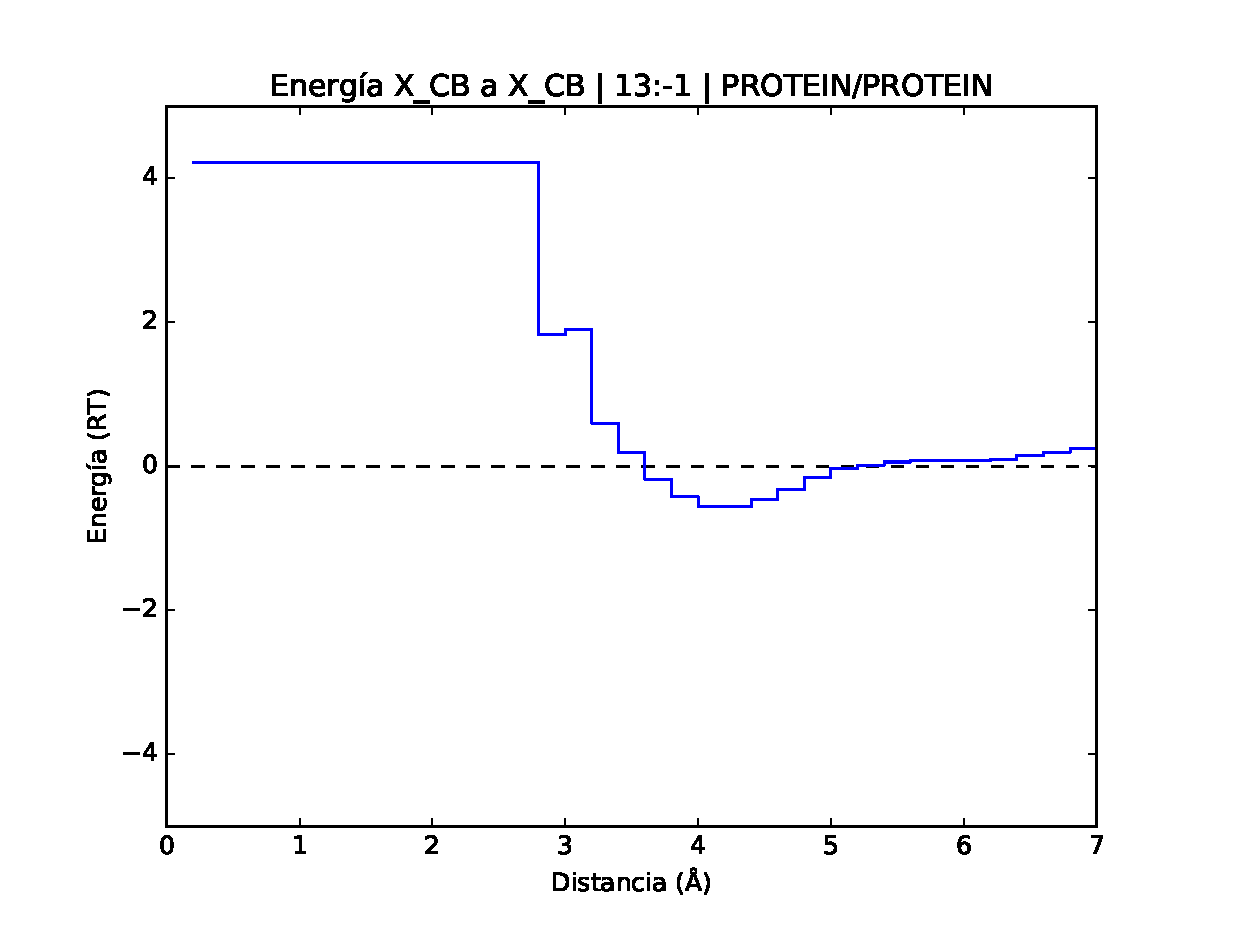
\includegraphics[width=\textwidth]{figures/prot_pot/dd/cb2cb.eps}
\caption{}
\end{subfigure}

\begin{subfigure}{.8\textwidth}
\centering
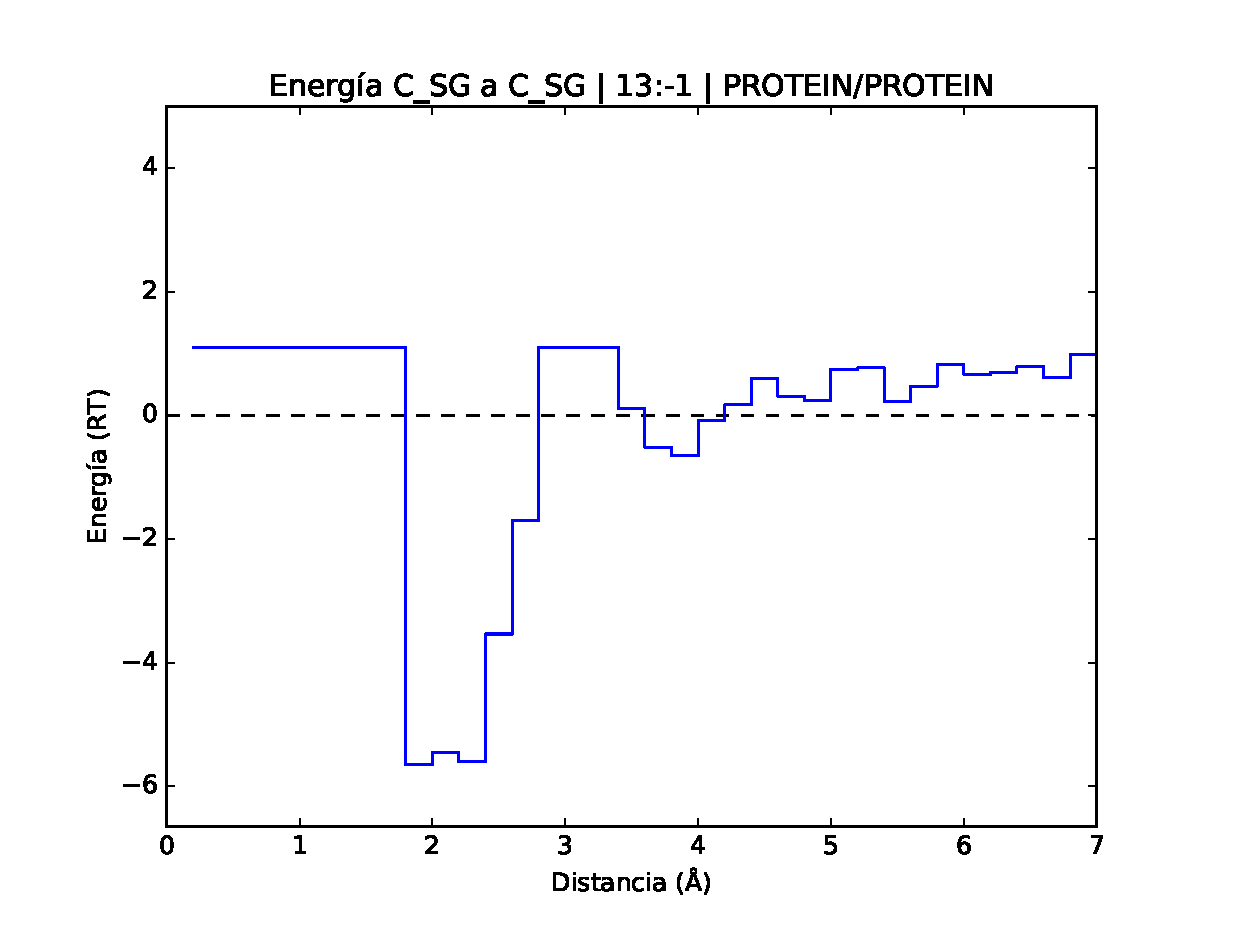
\includegraphics[width=\textwidth]{figures/prot_pot/dd/sh2sh.eps}
\caption{}
\end{subfigure}
\caption[Ejemplos de funciones de energía en proteínas]{Gráficos de las funciones de energía utilizadas en proteínas. 
En (a) se observa la energía (unidades RT) en función de la distancia en \si{\angstrom} para los carbonos beta de todos los aminoácidos. 
En (b) se tiene la función de energía para los átomos de azufre de císteina, representando los puentes disulfuro.}
\label{fig:energy1}
\end{figure}

\begin{figure}[p]
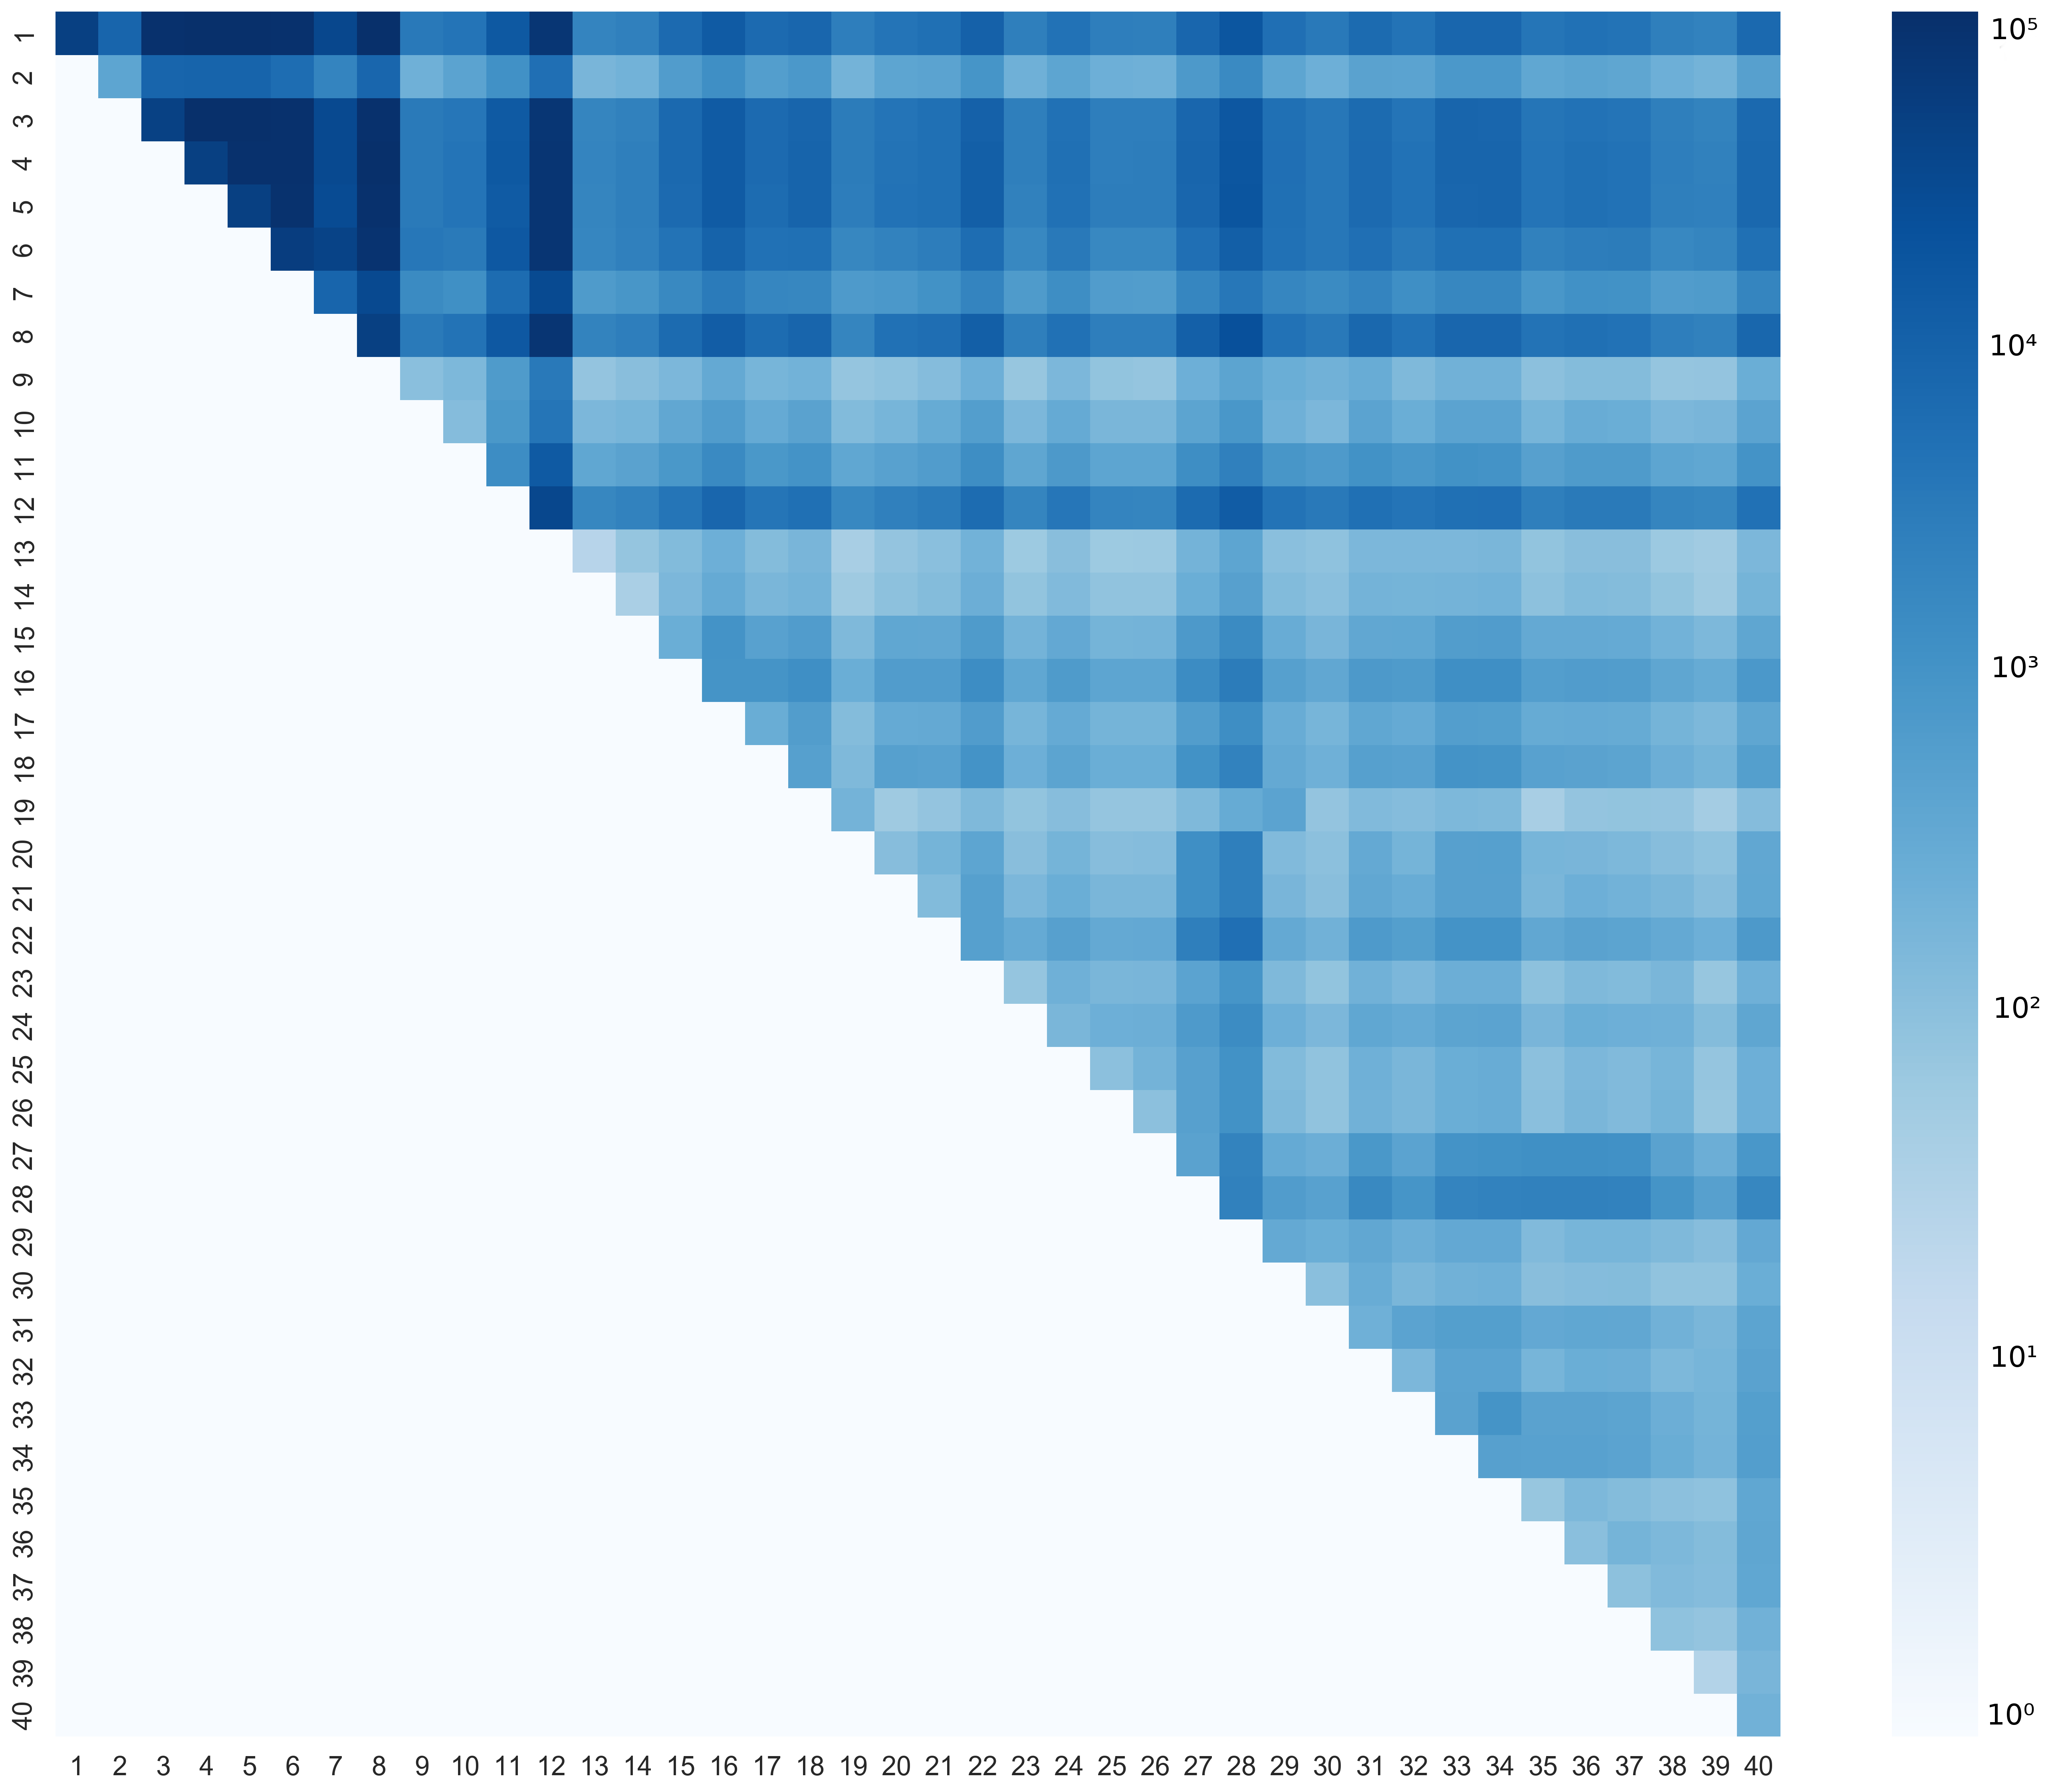
\includegraphics[width=\textwidth]{figures/prot_pot/mij.png}
\caption[Matriz de conteo para el cálculo del factor $\sigma$]{Matriz de conteo de interacciones para los potenciales en proteína, o \textit{Mij}. 
Solo se usa el triángulo superior de esta estructura, ya que no se considera el orden de las interacciones. 
Conteos están en escala logarítmica para facilitar la visualización.}
\label{fig:mij}
\end{figure}
\cleardoublepage

\subsubsection{Derivación de potenciales basados en conteos de átomos}
\par
Estos potenciales están basados en el conteo de la cantidad de centros atómicos dentro de un rango de 7 \si{\angstrom} de un átomo.
Las frecuencias están basadas en clases de 20 unidades con un máximo de 100 para todos los tipos de potenciales utilizados (ADN, ARN, proteínas).
Como no dependen de interacciones entre pares de átomos o distancias de residuos, se debe modificar la ecuación~\ref{ec:finalboltz}:

\begin{equation}
\Delta E^{i}(c) = RT\log \left[1 + M_{i}\sigma\right] - RT\log \left[ 1 + M_{i}\sigma \frac{f^{i}(c)}{f_{rel}} \right] \label{ec:surfboltz}
\end{equation}

Donde \textit{i} indica el tipo de átomo, \textit{Mi} es la cantidad de observaciones del átomo tipo \textit{i}, \textit{$f^{i}(c)$} es la frecuencia de observaciones en que un átomo \textit{i} tuvo \textit{c} átomos a su alrededor y \textit{$f_{rel}$} es la frecuencia esperada, equivalente a 1/(número de clases).
El factor de corrección $\sigma$ se mantiene en 1/50.
Un ejemplo de funciones de energía puede ser visto en la figura~\ref{fig:inteng}, donde se muestra la energía en función de la cantidad de átomos alrededor para un carbono aromático y para un nitrógeno ácido.
La metodología de derivación tiene pequeños cambios aparte de utilizar la ecuación~\ref{ec:surfboltz}.
En el algoritmo~\ref{alg:intpot} se tienen los pasos para la derivación, donde podemos notar los cambios respecto al algoritmo~\ref{alg:deralgo1}.
\textit{Mij} pasa a ser \textit{Mi}, una lista con la cantidad de observaciones de cada tipo de átomo, \textit{Fij} pasa a ser \textit{Fi}, una única tabla con las frecuencias de cada átomo \textit{i} para cada \textit{bin} de conteo, y \textit{Fxx} pasa a ser un único valor, \textit{Frel}.

\begin{algorithm}[H]
\caption{Pasos para la derivación de un potencial de conteo a partir de una lista de archivos PDB}\label{alg:intpot}
\begin{algorithmic}[1]
\Procedure{GenerateCountPotential}{}
\State $ \text{matrix1D } Mi $ \Comment{Vector de conteo de átomos del tipo I en la base de datos}
\State $ \text{matrix2D } Fi $ \Comment{Tabla de frecuencias de conteo para cada tipo atómico y \textit{bin}}
\State $ \text{float } Frel $ \Comment{Frecuencia esperada, 1/clases }
\State $ \text{list } pdblist \gets \text{GetPDBs}(argv1) $ \Comment{Carga estructuras PDB desde lista de archivos en disco}
\For {$ \textit{pdbstruct} \text{ in } \textit{PDBlist} $}
\State $ \text{CountEnv}(pdbstruct,Radius) $ \Comment{Calcula los átomos alrededor de otro átomo dentro del rango \textit{Radius}}
\EndFor
\State $ \text{CountCalculateIntFreq}(PDBlist,Fi,Frel,Mi,Nclases) $ \Comment{Calcula todas las tablas necesarias para la derivación del potencial}
\State $ \text{WritePotentialCount}(Fi,Frel,Mi,Nclases,Sigma) $ \Comment{Escribe el potencial creado a disco}
\EndProcedure
\end{algorithmic}
\end{algorithm}


\begin{figure}[p]
\centering
\begin{subfigure}{.8\textwidth}
\centering
\includegraphics[width=\textwidth]{figures/prot_pot/coarse/aromatic.eps}
\caption{}
\end{subfigure}

\begin{subfigure}{.8\textwidth}
\centering
\includegraphics[width=\textwidth]{figures/prot_pot/coarse/nh_acids.eps}
\caption{}
\end{subfigure}
\caption[Ejemplos de funciones de energía para conteo de átomos en proteínas]{En (a) se puede observar la energía en función del conteo de átomos en un rango de 7 \si{\angstrom} para carbonos aromáticos en proteínas. En (b) se puede observar otra función, pero para nitrógenos ácidos de los aminoácidos asparagina y glutamina.}
\label{fig:inteng}
\end{figure}
\cleardoublepage

\subsection{Cálculo de la superficie accesible al solvente de una molécula}
\par
Para el cálculo de la superficie accesible al solvente o SASA se utilizó el llamado algoritmo de Shrake y Rupley (\cite{Shrake1973}), descrito en el algoritmo~\ref{alg:shrkrply1}. Este consiste generar para cada átomo de una estructura una nube de puntos con forma esférica que están a una distancia de radio de Van der Waals más el radio de una molécula de una molécula de agua del centro del átomo. 
Cada punto representa un área equivalente al área de una esfera con el radio descrito anteriormente dividido por el número de puntos.
Al eliminar los puntos que se encuentran en el interior del volumen de las nubes de puntos de otros átomos, es posible obtener la superficie accesible al contar los puntos restantes y multiplicarlos por el valor de superficie que representan.
En la figura~\ref{fig:thomsonfig} se pueden observas las divisiones del área de una esfera que estos puntos representan.
\par
La nube de puntos debe tener todos sus puntos lo más equidistantes posible en el plano esférico para que el cálculo de superficie no tenga sesgos debido a la distribución desbalanceada de los puntos.
Esto se logró utilizando nubes de puntos precalculadas utilizando el por el software Thomson Applet (\cite{Saff1997,thomson}) de 15092 puntos. 

\begin{algorithm}[H]
\caption{Pasos para la obtención del SASA de una estructura }\label{alg:shrkrply1}
\begin{algorithmic}[1]
\Procedure{CalculateSASA}{}
\State $ \text{pdbstrudct } pdb $ \Comment{Estructura PDB}
\State $ \text{matrix2D } unitsphere $ \Comment{Matriz de 3xN con las coordenadas 3D de la nube de puntos en una esfera unitaria}
  \For {$ \textit{atomI} \text{ in } \textit{pdbstruct} $}
    \State $ \text{matrix2D } points \gets unitsphere * (atom.vdw + 1.4) + atom.coords $ \Comment{Escala y mueve una copia de la nube de N puntos a las coordenadas del átomo actual}
    \State $ \text{int } surfacepoints \gets N $ \Comment{Contador de puntos expuestos al solvente}
    \State $ \text{float } totalSASA \gets 0 $ \Comment{Superficie expuesta final}
    \For{$  \textit{atomJ} \text{ in } \textit{atomI.interactions}  $} \Comment{Itera sobre los átomos J que interactuan con I}
      \For{$  \textit{point} \text{ in } \textit{points}  $}
        \If {$\text{IsPointInVolume}(atomJ,point) \text{ and } point.enabled$} \Comment{Revisa si el punto esta adentro del volumen del átomo J y si no fue contado antes}
          \State $ surfacepoints -= 1  $ \Comment{Decrementa el contador de puntos}
          \State $ point.enabled = False $ \Comment{Desabilita el punto, ya que no es necesario volver a revisarlo}
        \EndIf
      \EndFor
    \EndFor
    \State $ atomI.SASA \gets surfacepoints * atomI.tAREA / N $ \Comment{Calcula área del átomo}
    \State $ totalSASA \gets atomI.SASA + totalSASA $ \Comment{Suma el área al área total}
  \EndFor
\State $ \Return \textit{ totalSASA } $ \Comment{Retorna el SASA final}

\EndProcedure
\end{algorithmic}
\end{algorithm}

\begin{figure}[p]
\centering
\centering
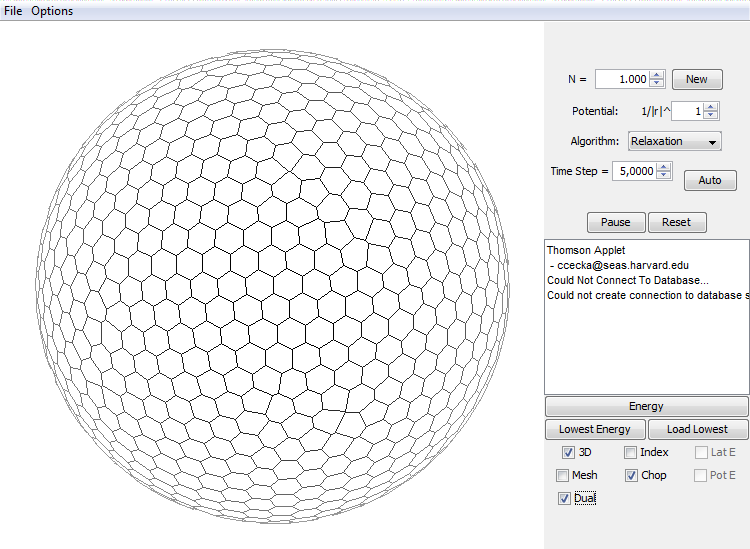
\includegraphics[width=\textwidth]{figures/thomson/thomson.png}
\caption[Esfera en el software Thomson Applet]{En este ejemplo podemos observar una esfera subdividida en 1000 áreas equivalentes. Inicialmente las subáreas son inicializadas con valores aleatorios, los cuáles son optimizados utilizando un algoritmo de relajación considerando cada punto como una carga eléctrica forzada a moverse sobre una esfera.}
\label{fig:thomsonfig}
\end{figure}
\cleardoublepage

\subsection{Cálculo de las subsuperfícies de interacción}
\par
Para calcular las subsuperfícies de interacción entre dos átomos, se debe extender el algoritmo~\ref{alg:shrkrply1}.
Esto se hace agregando nuevas variables para almacenar la información de que átomos entierran un cierto punto en la superficie de otro.
Así es posible encontrar los grupos de puntos de un átomo que son enterrados por otros grupos únicos de átomos, identificando así todos los sobrelapamientos únicos posibles, como indicado en el diagrama de la figura~\ref{fig:dbsa1}.
En el algoritmo~\ref{alg:dbsa} podemos ver las modificaciones, donde se agregan las estructuras \textit{pBuriedBy} y \textit{AreaBuriedBy}, que permiten almacenar la información de que puntos de la superficie de un átomo son enterrados por cuáles otros grupos de átomos. 
La estructura final, \textit{AreaBuriedBy} contiene los conjuntos únicos de átomos y la cantidad de puntos que cada uno de los conjuntos entierra.
\par
En la figura~\ref{fig:dbsa1} tenemos el ejemplo más simple donde ocurren sobrelapamientos, un sistema de 3 cuerpos.
Para este sistema, la superficie enterrada del cuerpo 1 por el cuerpo 2 corresponde a la sección en rojo, más la sección en púrpura dividida por 2.
Esto se debe a que dos átomos participan en este sobrelapamiento, que incluye el cuerpo 2.
Por lo tanto, el valor de superficie enterrada que un cuerpo \textit{B} le causa a un cuerpo \textit{A} es igual a la suma de todos los sobrelapamientos divididos por la cantidad de átomos participantes donde se encuentra el cuerpo \textit{B}.


\begin{algorithm}[H]
\caption{Pasos para el cálculo de las superficies de interacción }\label{alg:dbsa}
\begin{algorithmic}[1]
\Procedure{CalculateDBSA}{}
\State $ \text{pdbstrudct } pdb $ \Comment{Estructura PDB}
\State $ \text{matrix2D } unitsphere $ \Comment{Matriz de 3xN con las coordenadas 3D de la nube de puntos en una esfera unitaria}
  \For {$ \textit{atomI} \text{ in } \textit{pdbstruct} $}
    \State $ \text{map } pBuriedBy  $ \Comment{Almacena las listas de átomos que entierran un cierto punto en la superfice del átomo \textit{I}}
    \State $ \text{list } AreaBuriedBy $ \Comment{Almacena los conjuntos de átomos únicos encontrados y la cantidade puntos que entierran} 
    \State $ \text{matrix2D } points \gets unitsphere * (atom.vdw + 1.4) + atom.coords $ \Comment{Escala y mueve una copia de la nube de N puntos a las coordenadas del átomo actual}
    \For{$  \textit{atomJ} \text{ in } \textit{atomI.interactions}  $} \Comment{Itera sobre los átomos J que interactuan con I}
      \For{$  \textit{point} \text{ in } \textit{points}  $}
        \If {$\text{IsPointInVolume}(atomJ,point) $} \Comment{Revisa si el punto esta adentro del volumen del átomo J}
          \State $ pBuriedBy[point].\text{add}(\textit{atomJ})  $ \Comment{Agrega átomo a la lista de átomos que entierran este punto}
        \EndIf
      \EndFor
    \EndFor
    \State $ \textit{AreaBuriedBy} \gets \text{ParseSets}(pBuriedBy) $ \Comment{Procesa los conjuntos encontrados y calcula el área enterrada por cada uno}
    \State $ \textit{atomI}.AreaBuriedBy \gets \textit{AreaBuriedBy} $ \Comment{Almacena las interacciones en el objeto átomo}
  \EndFor
\EndProcedure
\end{algorithmic}
\end{algorithm}

\begin{figure}[p]
\centering
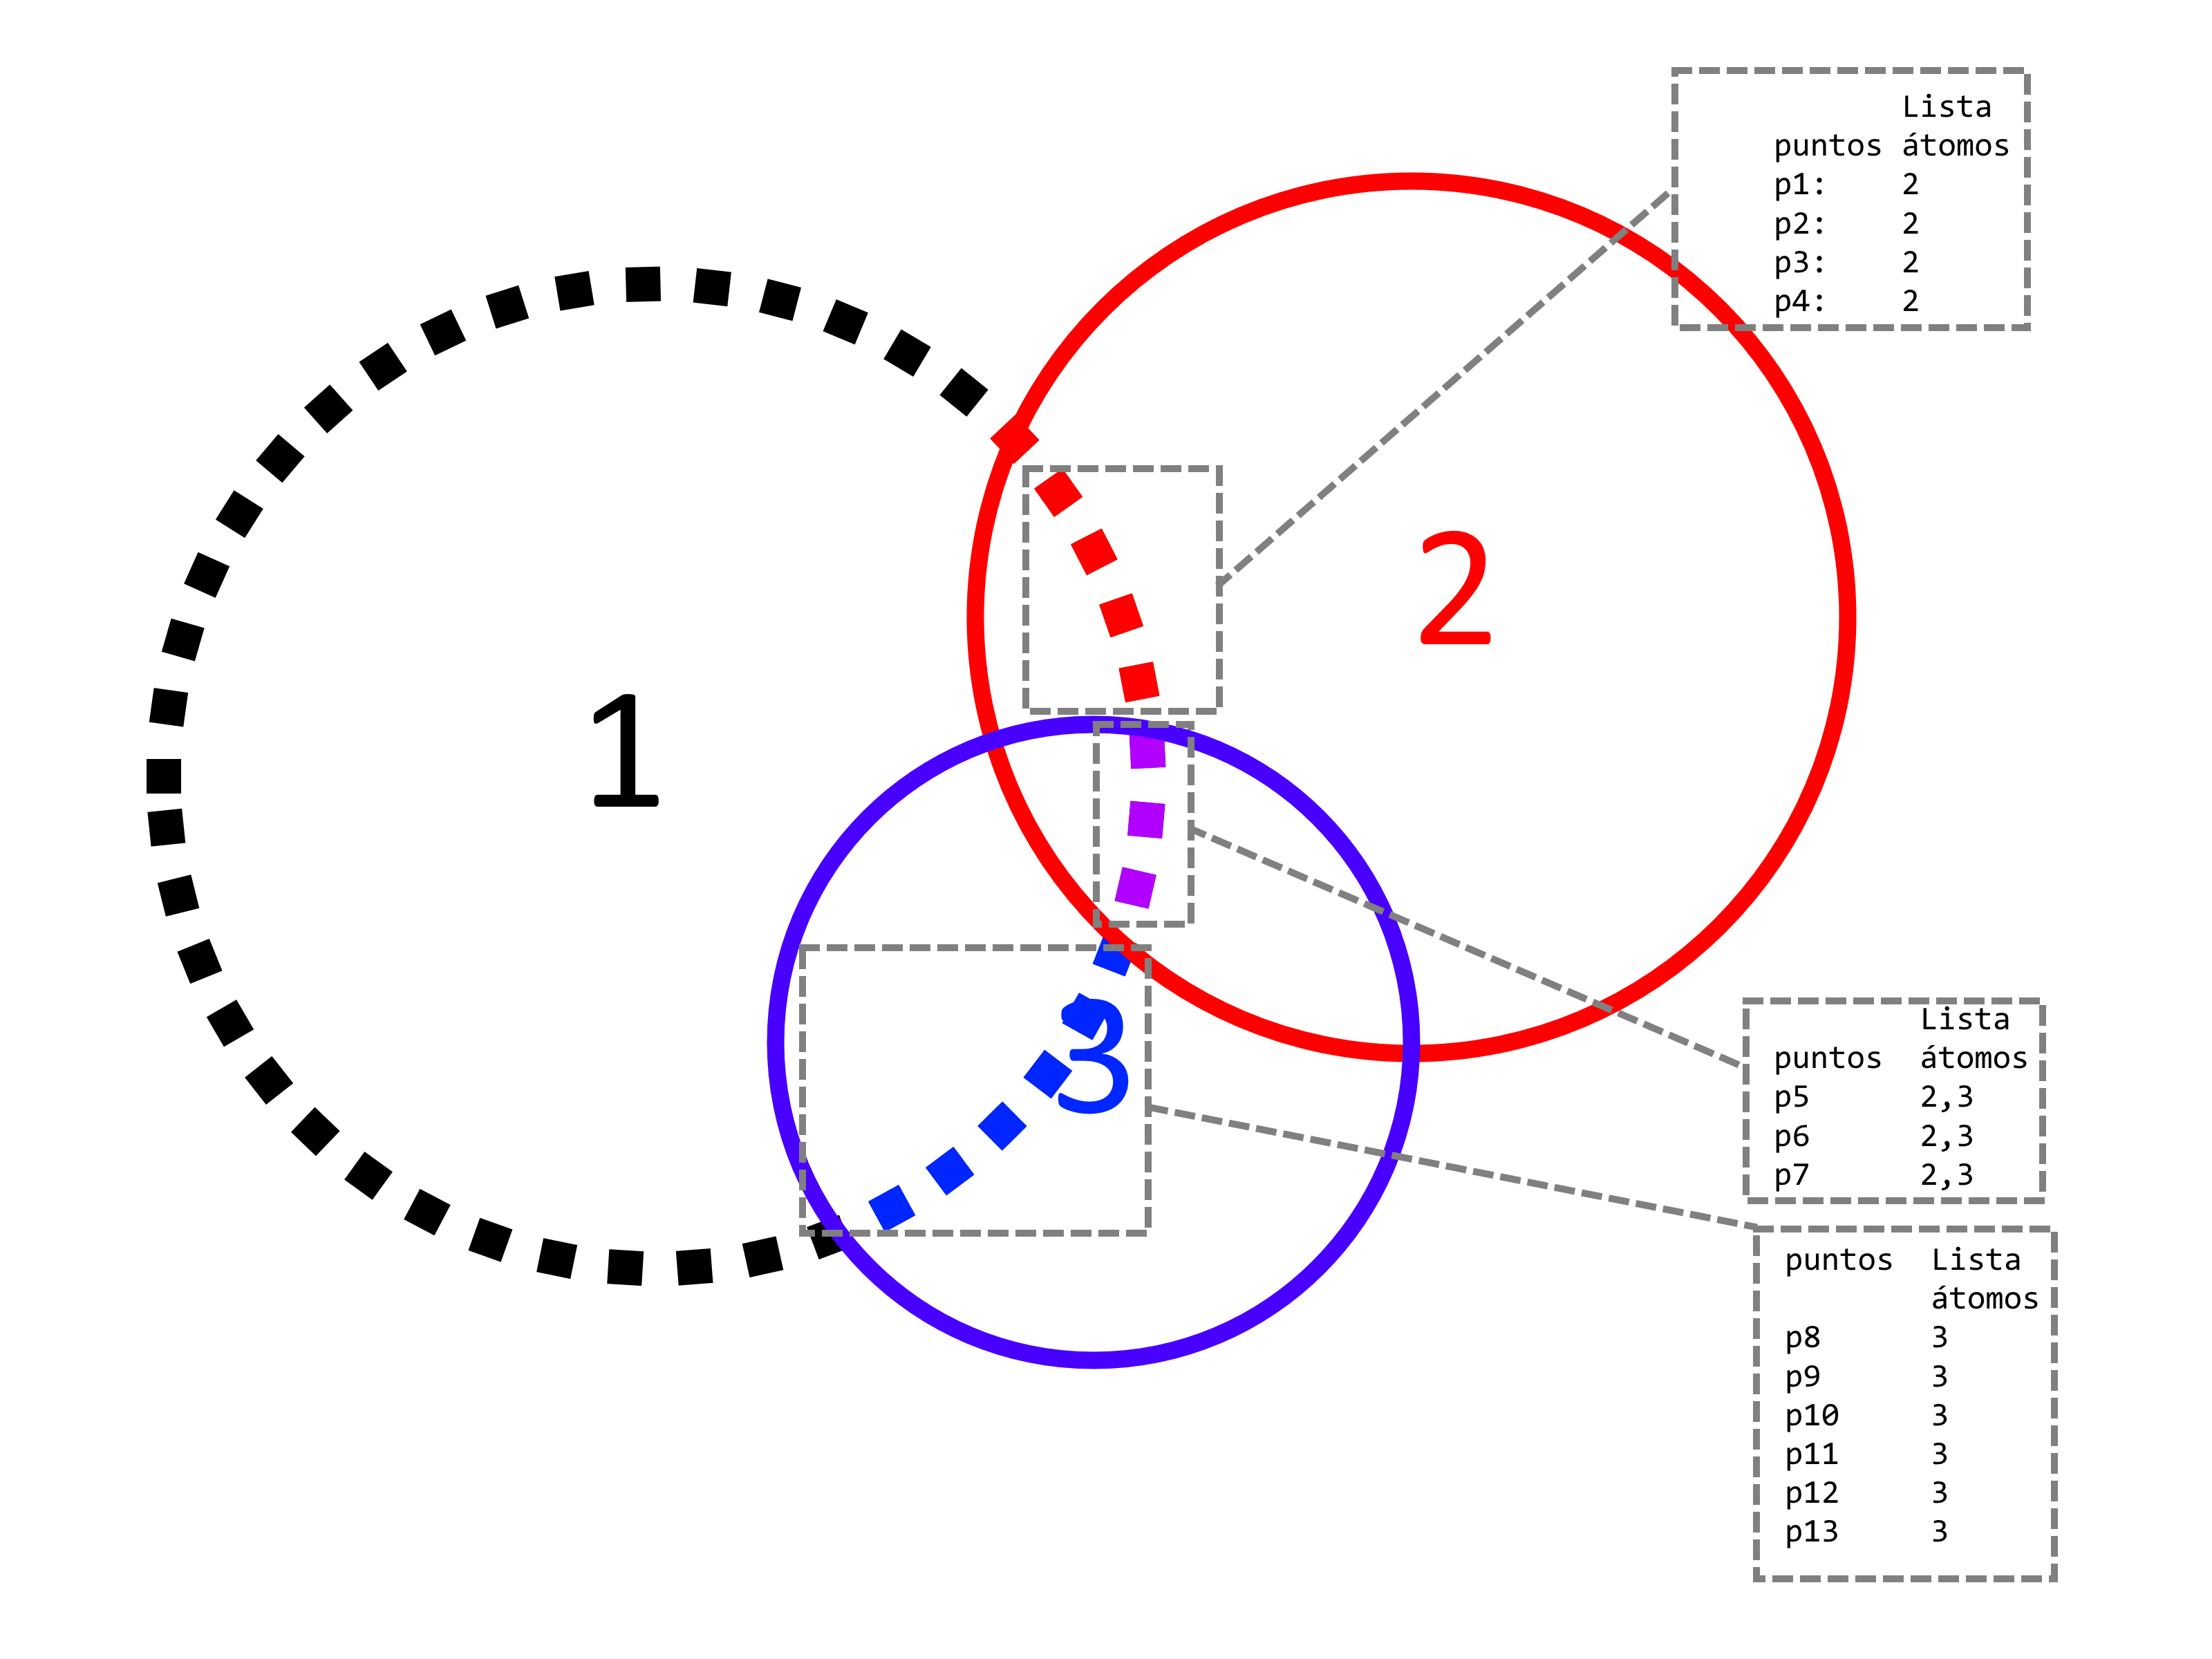
\includegraphics[width=\textwidth]{figures/dbsa.png}
\caption[Cálculo de subsuperfices de interacción]{Diagrama en 2D del funcionamiento del algoritmo para el cálculo de las subsuperficies de interacción. En este ejemplo de 3 cuerpos, se observa como el cuerpo 1 tiene su superfície enterrada por los cuerpos 2 y 3. Cada punto en la superficie de 1 representa un valor de superficie equivalente a (superfície total)/(número de puntos). Los puntos coloreados de rojo representan el área enterrada solo por el cuerpo 2, los puntos azules el área enterrada solo por 3, y los puntos púrpuras el área enterrada por los cuerpos 2 y 3. En los recuadros grises se tienen representaciones del mapa de puntos enterrados hacia lista de átomos, \textit{pBuriedBy} en el algoritmo~\ref{alg:dbsa}.}
\label{fig:dbsa1}
\end{figure}
\cleardoublepage

\subsection{Derivación de potenciales basados en BSA}
\par
Al obtener los valores de \si{\angstrom}\textsuperscript{2}  para cada interacción entre átomos \textit{I} y \textit{J}, la derivación de un potencial procede de manera similar a los potenciales que utilizan distancia.
Un detalle importante es que dado que los radios de Van der Waals de los átomos \textit{I} y \textit{J} pueden ser distintos, lo que puede causar que el valor de superficie que \textit{I} entierra de \textit{J} sea distinto al valor que \textit{J} entierra de \textit{I}.
Para resolver este problema, se derivan dos potenciales al mismo tiempo, uno con los valores de \textit{I} que entierran a \textit{J} y otro para los valores de \textit{J} que entierran a \textit{I}.
Estos dos potenciales se evalúan y suman al evaluar cualquier interacción de \textit{I} contra \textit{J}.

\subsection{Derivación de potenciales basados en SASA}
\par
Los potenciales basados en SASA se derivan de la misma manera que los potenciales de conteos de átomos.
El único cambio el uso del SASA de cada átomo, en vez del número de átomos alrededor, como la variable en todas las ecuaciones y funciones.
Los parámetros utilizados para estos potenciales fueron 30 clases de 1.67 \si{\angstrom}\textsuperscript{2} con el límite de la última clase en 50 \si{\angstrom}\textsuperscript{2}.
Estos parámetros se usaron para los potenciales en proteínas, ADN y ARN.
En la figura~\ref{fig:sasapots} se pueden observar los dos potenciales SASA, uno para átomos de carbono hidrofóbicos y otro para nitrógenos hidrofílicos.

\begin{figure}[p]
\centering
\begin{subfigure}{.8\textwidth}
\centering
\includegraphics[width=\textwidth]{figures/prot_pot/sasa/sasa_arom.eps}
\caption{}
\end{subfigure}
\begin{subfigure}{.8\textwidth}
\centering
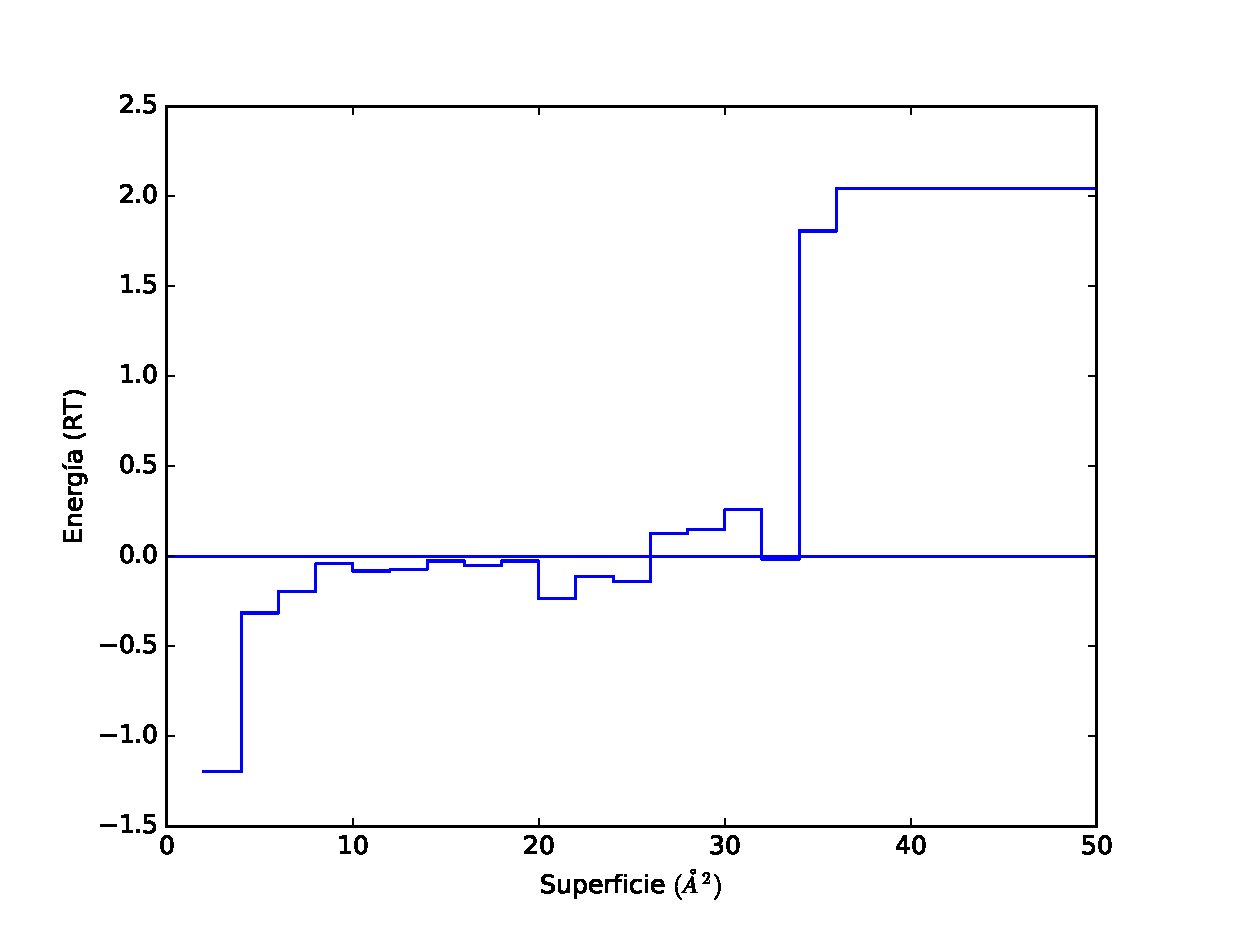
\includegraphics[width=\textwidth]{figures/prot_pot/sasa/sasa_n_hist.eps}
\caption{}
\end{subfigure}
\caption[Ejemplos de funciones de energía SASA en proteínas]{En (a) se puede observar la energía en función de la superficie expuesta al solvente para átomos de carbono aromáticos. En (b) se puede observar otra función, pero para nitrógenos terminales de histidina}
\label{fig:sasapots}
\end{figure}

\subsection{Combinación de los potenciales de distancia y conteo}
\par
Estos potenciales se combinan con la siguiente formula, que es ejecutada con los valores de energía para cada átomo encontrado. 
Esta suma los valores de los potenciales de distancia y conteo, utilizando un peso \textit{$W_{it}$} que depende del tipo molecular al que pertenece el átomo, de su tipo atómico, y de la cantidad de interacciones con otros átomos que posee. (\cite{Melo1997})

\begin{equation}
E_{ti} = E^{DD}_{i} + (E^{CNT}_{i} * W_{ti})
\end{equation}
Donde:
\[W_{ti} = \left\{
\begin{array}{ll}
(Imax_{t} - C_{i} - 1)/(Imax_{t} - Imin_{ti} - 1) & C_{i} < Imax_{t} \\
0 & C_{i} \geq Imax_{t} \\
\end{array}
\right. \]
Los términos \textit{Imax}, \textit{C}, e \textit{Imin} corresponden respectivamente al número máximo de interacciones encontrado para el tipo molecular correspondiente en el conjunto de entrenamiento, el número de interacciones que posee el átomo evaluado, y el número mínimo de interacciones encontradas para el tipo atómico y molecular evaluado.
Los términos $E^{DD}$ y $E^{CNT}$ corresponden a las energías calculados por los potenciales de distancia y conteo respectivamente.

\subsection{Combinación de los potenciales BSASA y SASA}

Se utiliza la misma fórmula descrita para la combinación de los potenciales de distancia y conteo.

\subsection{Cálculo del IP (\textit{Information Product})}
\par
El IP o \textit{Information Product} es una medida de la información mutua de un potencial (\cite{Solis2008}), que permite la comparación de estos de manera independiente a pruebas usando estructuras.
Esta basado en la siguiente ecuación:
\begin{equation}
P = \sqrt{\overline{n}}\cdot\Delta\overline{E}^{ij} \label{ec:ip}
\end{equation}
Donde $ \overline{n} $ es el número promedio de observaciones de interacciones válidas de acuerdo a los parámetros del potencial en el conjunto de estructuras de derivación del mismo mientras que $ \Delta\overline{E}^{ij} $ es el valor promedio de energía de estas mismas interacciones. En los potenciales de conteo y SASA el término \textit{ij} pasa a ser solo \textit{i}.

